\documentclass[11pt,usenames]{article}
\usepackage{srcltx,pdfsync}
%\usepackage[pdflatex=false,recompilepics]{gastex} 
\usepackage{amsmath,amssymb,amsfonts}
\usepackage{color}
\usepackage{hyperref, url}
\usepackage{geometry}
\usepackage{graphicx,subfigure,wrapfig}
\geometry{verbose,a4paper,tmargin=30mm,bmargin=50 mm,lmargin=25mm,rmargin=16mm}
\usepackage{ifthen}

\def\Lap{\ensuremath{\mathcal{L}}}
\usepackage{fancyhdr}
\pdfpagewidth 8.5in
\pdfpageheight 11in

\pagestyle{fancy}
\headheight 35pt

\usepackage{listings} % For inserting Code
\usepackage{color} %red, green, blue, yellow, cyan, magenta, black, white
\definecolor{mygreen}{RGB}{28,172,0} % color values Red, Green, Blue
\definecolor{mylilas}{RGB}{170,55,241}


\graphicspath{{./Images/}}

%%%%%%%%%%%%%
\usepackage[fancythm]{jphmacros2e}
\renewcommand{\footrulewidth}{0.5 pt}

\rhead{\small{ML Project Task 1 Report}}
\chead{}
\lhead{\small{CAP 6610}}
\lfoot{Ninad Gaikwad - 41482960}
\cfoot{\thepage}
\rfoot{}

\title{}

\date{}


\begin{document}
	
% Formatting for the required code	
	\lstset{language=Matlab,%
		%basicstyle=\color{red},
		breaklines=true,%
		morekeywords={matlab2tikz},
		keywordstyle=\color{blue},%
		morekeywords=[2]{1}, keywordstyle=[2]{\color{black}},
		identifierstyle=\color{black},%
		stringstyle=\color{mylilas},
		commentstyle=\color{mygreen},%
		showstringspaces=false,%without this there will be a symbol in the places where there is a space
		numbers=left,%
		numberstyle={\tiny \color{black}},% size of the numbers
		numbersep=9pt, % this defines how far the numbers are from the text
		emph=[1]{for,end,break},emphstyle=[1]\color{red}, %some words to emphasise
		%emph=[2]{word1,word2}, emphstyle=[2]{style},    
	}
% Formatting for the required code
	
	\begin{center}
		{\sc ML Project Task 1 Report}\\
		University of Florida \\
		Computer \& Information Science Engineering
		\vspace{0.5 cm}
	\end{center}
	
	{\large \begin{center}
			\textbf{Project - Task 2-3 Combined Report}\\
			GAN and VAE for Handwriting Recognition
	\end{center}}
	
	
	%\newpage
	
	
	%\tableofcontents
	
	
	\newpage
	
	
	\section{Network Model Architecture:}\label{section:NetworkModelArchitecture}

	\subsection{GAN Architecture:}\label{subsection:GAN_NetworkModelArchitecture}
	The generator model of the GAN includes one dense layer followed by two convolutional layers.
	
	\subsection{VAE Architecture:}\label{subsection:VAE_NetworkModelArchitecture}
	The encoder model of the VAE includes two convolutional layers followed by a dense layer.	
	
	\section{Training Data for the Models:}\label{section:TrainingDatas}
	MINST Dataset	
	
	\section{Training Results:}\label{section:TrainingResults}
	
	\subsection{GAN Results:}\label{subsection:GAN_Results}
	
	\begin{figure}[htpb]
		\centering
		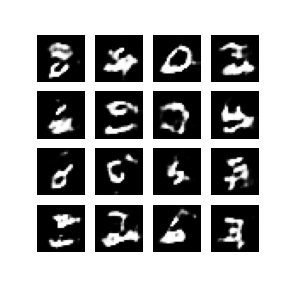
\includegraphics[scale=1]{GAN_image_at_epoch_0001.png}
		\caption{GAN Result}
		\label{fig:FigureLabel1}
	\end{figure}

	\subsection{VAE Results:}\label{subsection:VAE_Results}	
	\begin{figure}[htpb]
		\centering
		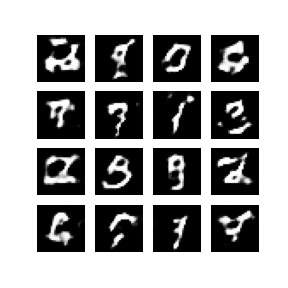
\includegraphics[scale=1]{GAN_image_at_epoch_0002.png}
		\caption{VAE Result}
		\label{fig:FigureLabel1}
	\end{figure}	
	
	\section{Analysis of Results:}\label{section:AnalysisResults}
	
	\subsection{GAN Analysis:}\label{subsection:GAN_Analysis}
	The GAN has not performed well. The reason for this is small training data sample, simple structure of the generator and discriminator nets and the dimensionality of the noise. To improve performance, all the above have to be tuned properly, along with the filter value of the convolutional nets.

	\subsection{VAE Analysis:}\label{subsection:VAE_Analysis}			
	The VAE has not performed well. The reason for this is small training data sample, simple structure of the encoder and the decodser nets and the dimensionality of the latent variable. To improve performance, all the above have to be tuned properly along with the filter value of the convolutional nets.	
		
		%\bibliographystyle{IEEEtran}
		%\bibliography{{./BiBFolder/BibFile}}	
	
\end{document}

		\begin{table}[htpb]
	\caption{Performance comparison of baseline and proposed controller.}
	\label{tab:TableLabel}
	\begin{center}
		\begin{tabular}{|c|c|c|c|}
			\hline
			& Baseline & Proposed & a \\
			\hline
			Refrigerator temp. violation ($hours/Day$) & 7.1250 & 0.0416 & b\\
			\hline
			Secondary loads not served (\% $time$) & 57 & 48.63 & c\\
			\hline
			Secondary loads not served (\% $time$) & 57 & 48.63 & c\\
			\hline								
		\end{tabular}
	\end{center}
\end{table} 


\begin{table}[htpb]
	\caption{Test Table.}
	\label{tab:TableLabel1}
	\begin{center}
		\begin{tabular}{|c | c | c |}
			\hline
			\textbf{1} & \textbf{2} & \textbf{3} \\
			\hline
			\hline
			4 & 5 & 6 \\
			\hline
			\hline
			7 & 8 & 9 \\
			\hline							
		\end{tabular}
	\end{center}
\end{table}	


	This is the figure.

\begin{figure}[htpb]
	\centering
	
\includegraphics[scale=0.25]{LatexIcon.png}
	\caption{Caption}
	\label{fig:FigureLabel1}
\end{figure}

The Fig~\ref{fig:FigureLabel1} is great.\\	


This is the figure.

\begin{figure}[htpb]
	\centering
	
\includegraphics[scale=0.25]{LatexIcon.png}
	\caption{Caption}
	\label{fig:FigureLabel}
\end{figure}

The Fig~\ref{fig:FigureLabel} is great.












